\makeglossaries

\newglossaryentry{Batch}
{
	name=Batch,
	description={Batch beziehungsweise Batch-Verarbeitung bezeichnet in der IT die sog. \glqq Stapelverarbeitung\grqq.
Das heißt, dass Programme mit minimalem menschlichen Eingreifen nacheinander abgearbeitet werden.
Beispielsweise meist zu einer vorher festgelegten Zeit, gesteuert wird dies über sog. \glqq Scheduling\grqq-Systeme.
Zum Beispiel wird einmal am Tag zu einer ganz bestimmten Uhrzeit die tägliche Bewertung\footnote{Beschreibung in Absatz \ref{sssec:täglbew}} der DATEV Rechnungsschreibung durchgeführt.
Die auszuführenden Programme laufen in sogenannten \glqq Batch-Jobs\grqq.
\cite{Ebbers.2011}}
}

\newglossaryentry{Batch-Job}
{
	name=Batch Job,
	description={In einem Batch\-Job, in dieser Arbeit wird \glqq Job\grqq{} gleichbedeutend verwendet, wird dem System mitgeteilt welches Programm mit welchen Ein- und Ausgabedateien und Parametern gestartet werden soll.
Die Skriptsprache, die diese Jobs definiert, ist im IBM-Mainframe-Umfeld die sog. \glqq Job Control Language\grqq, kurz JCL.
Die drei Grundbausteine der JCL werden im Folgenden beschrieben.\\
Zunächst ist \glqq JOB\grqq{} zu nennen, auch Jobkarte genannt.
Hier werden der Name des Jobs, Berechnungsinformationen, maximal zur Verfügung stehende CPU-Zeit und weitere Job-weite Parameter gesetzt.
Im Beispiel \ref{fig:jclBsp} Zeilennummer eins bis drei.\\
Innerhalb eines Jobs wird mit Hilfe des \glqq EXEC\grqq{} Befehls dem System mitgeteilt, welches Programm gestartet werden soll.
Es können mehrere \glqq EXEC\grqq{}  Befehle in einem Job vorkommen, dabei wird jeder einzelne als sogenannter \glqq Job step\grqq{} bezeichnet.
Dabei können dem Programm neben den Ein-/Ausgabedateien auch weitere Parameter übergeben werden.
Im Beispiel \ref{fig:jclBsp} Zeilennummer zehn.\\
Als letztes ist der \glqq DD\grqq{} Baustein zu nennen.
\glqq DD\grqq{} steht für Data Definition.
Ein DD-Statement verknüpft den sog. DD-Namen mit einer Datei oder einem I/O Gerät und ist somit ein Alias für diese.
Ein \glqq DD\grqq{} Baustein ist immer an ein \glqq EXEC\grqq{} Befehl gebunden.
Einem \glqq EXEC\grqq{} können mehrere \glqq DD\grqq{} Bausteine zugeordnet sein. 
Im Beispiel \ref{fig:jclBsp} Zeilennummer 12 bis 15 und 19.
Hier ist auch zu sehen, dass Daten auch Inline an ein DD-Statement übergeben werden kann.
\cite{Ebbers.2011}
\begin{figure}[h]
\centering
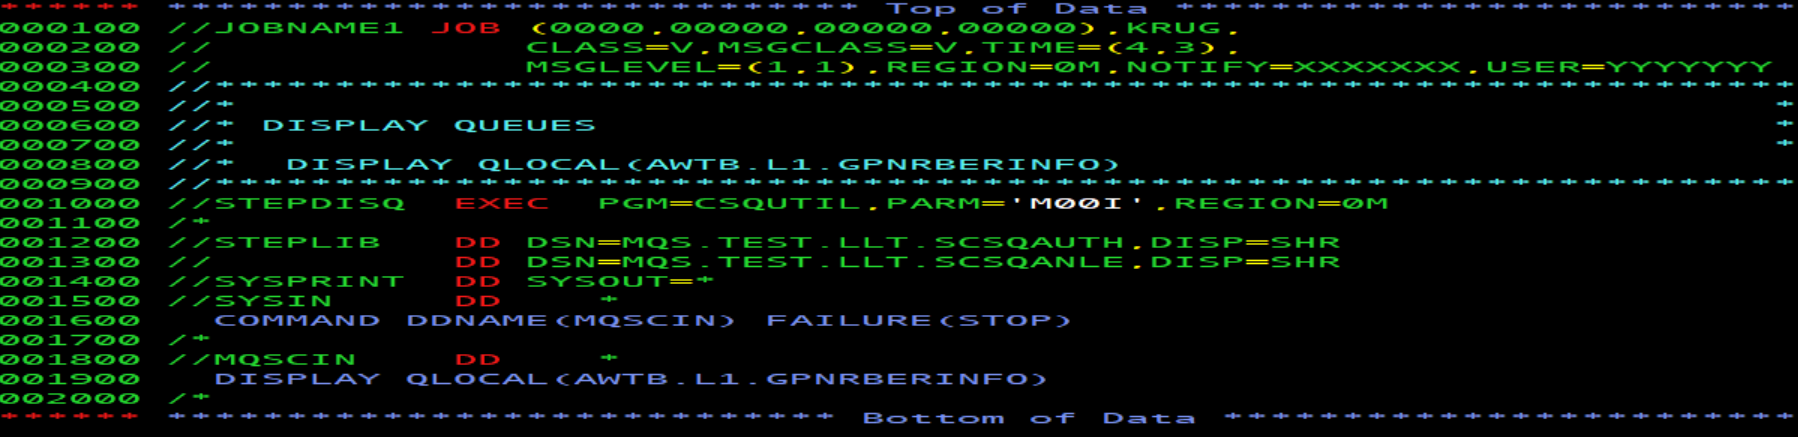
\includegraphics[width=\textwidth]{figures/dispq.PNG}
\caption{Job Beispiel, Display einer IBM MQ}
\label{fig:jclBsp}
\end{figure}}
}

\newglossaryentry{cloudcomp}
{
	name=Cloud-Computing,
	description={\glqq Cloud Computing bezeichnet das dynamisch an den Bedarf angepasste Anbieten, Nutzen und Abrechnen von IT-Dienstleistungen über ein Netz. Angebot und Nutzung dieser Dienstleistungen erfolgen dabei ausschließlich über definierte technische Schnittstellen und Protokolle. Die Spannbreite der im Rahmen von Cloud Computing angebotenen Dienstleistungen umfasst das komplette Spektrum der Informationstechnik und beinhaltet unter anderem Infrastruktur (z. B. Rechenleistung, Speicherplatz), Plattformen und Software.\grqq(Quelle: \cite{.23.2.2020b}}
}

\newglossaryentry{docker}
{
	name=Docker,
	description={Docker ist eine offene Plattform für die Entwicklung, Paketierung und Ausführen von Anwendungen auf verteilten Systemen. Zu diesen Systemen zählen unter anderem die Cloud, Datenzentren oder virtuelle Maschinen(Quelle: \cite{Vohra.2016}}
}

\newglossaryentry{vsam}
{
	name=VSAM,
	description={Virtual Storage Access Method, spezielle z/OS Dateiart, die schnelle I/O-Zugriffe ermöglicht.(Quelle: \cite[S. 2-4]{Lovelace.2013}}
}

\newglossaryentry{racf}
{
	name=RACF,
	description={Die Resource Access Control Facility, kurz RACF, ist ein externer Sicherheitsmanager für z/OS.
Dieser bietet eine Rechteverwaltung für das z/OS Betriebssystem an.
Damit werden unter anderem Zugriffsrechte auf Dateien und Subsysteme gesteuert.(Quelle: \cite[S. 18-21]{InternationalBusinessMachinesCorporation.2008}}
}

\newglossaryentry{rexx}
{
	name=REXX,
	description={Restructured Extended Executor versteht sich als Skriptsprache und kommt nicht nur am Mainframe zum Einsatz.
So kann es als Bindeglied für Betriebssystembefehle, grafischen Interfaces, Objekten, Funktionen und Serviceroutinen gesehen werden.
So wird es, wie auch in dieser Arbeit, unter anderem für die Automation von sich wiederholenden Systemadministrationsaufgaben eingesetzt.
\cite{Fosdick.2005}}
}